\providecommand{\main}{../../..}
\documentclass[\main/dresen_thesis.tex]{subfiles}

\begin{document}
  \section{Vibrating Sample Magnetometry (VSM)}
    \label{ch:methods:vsm}
    In vibrating sample magnetometry the macroscopic magnetization of a sample is determined by using Faraday's law of induction
    \begin{align}
      U \eq \frac{\dint }{\dint t} (BA),
    \end{align}
    which relates the voltage measured between the two ends of a wire loop with the change of the magnetic flux that passes through the wire with respect to time.
    \begin{figure}[tb]
      \centering
      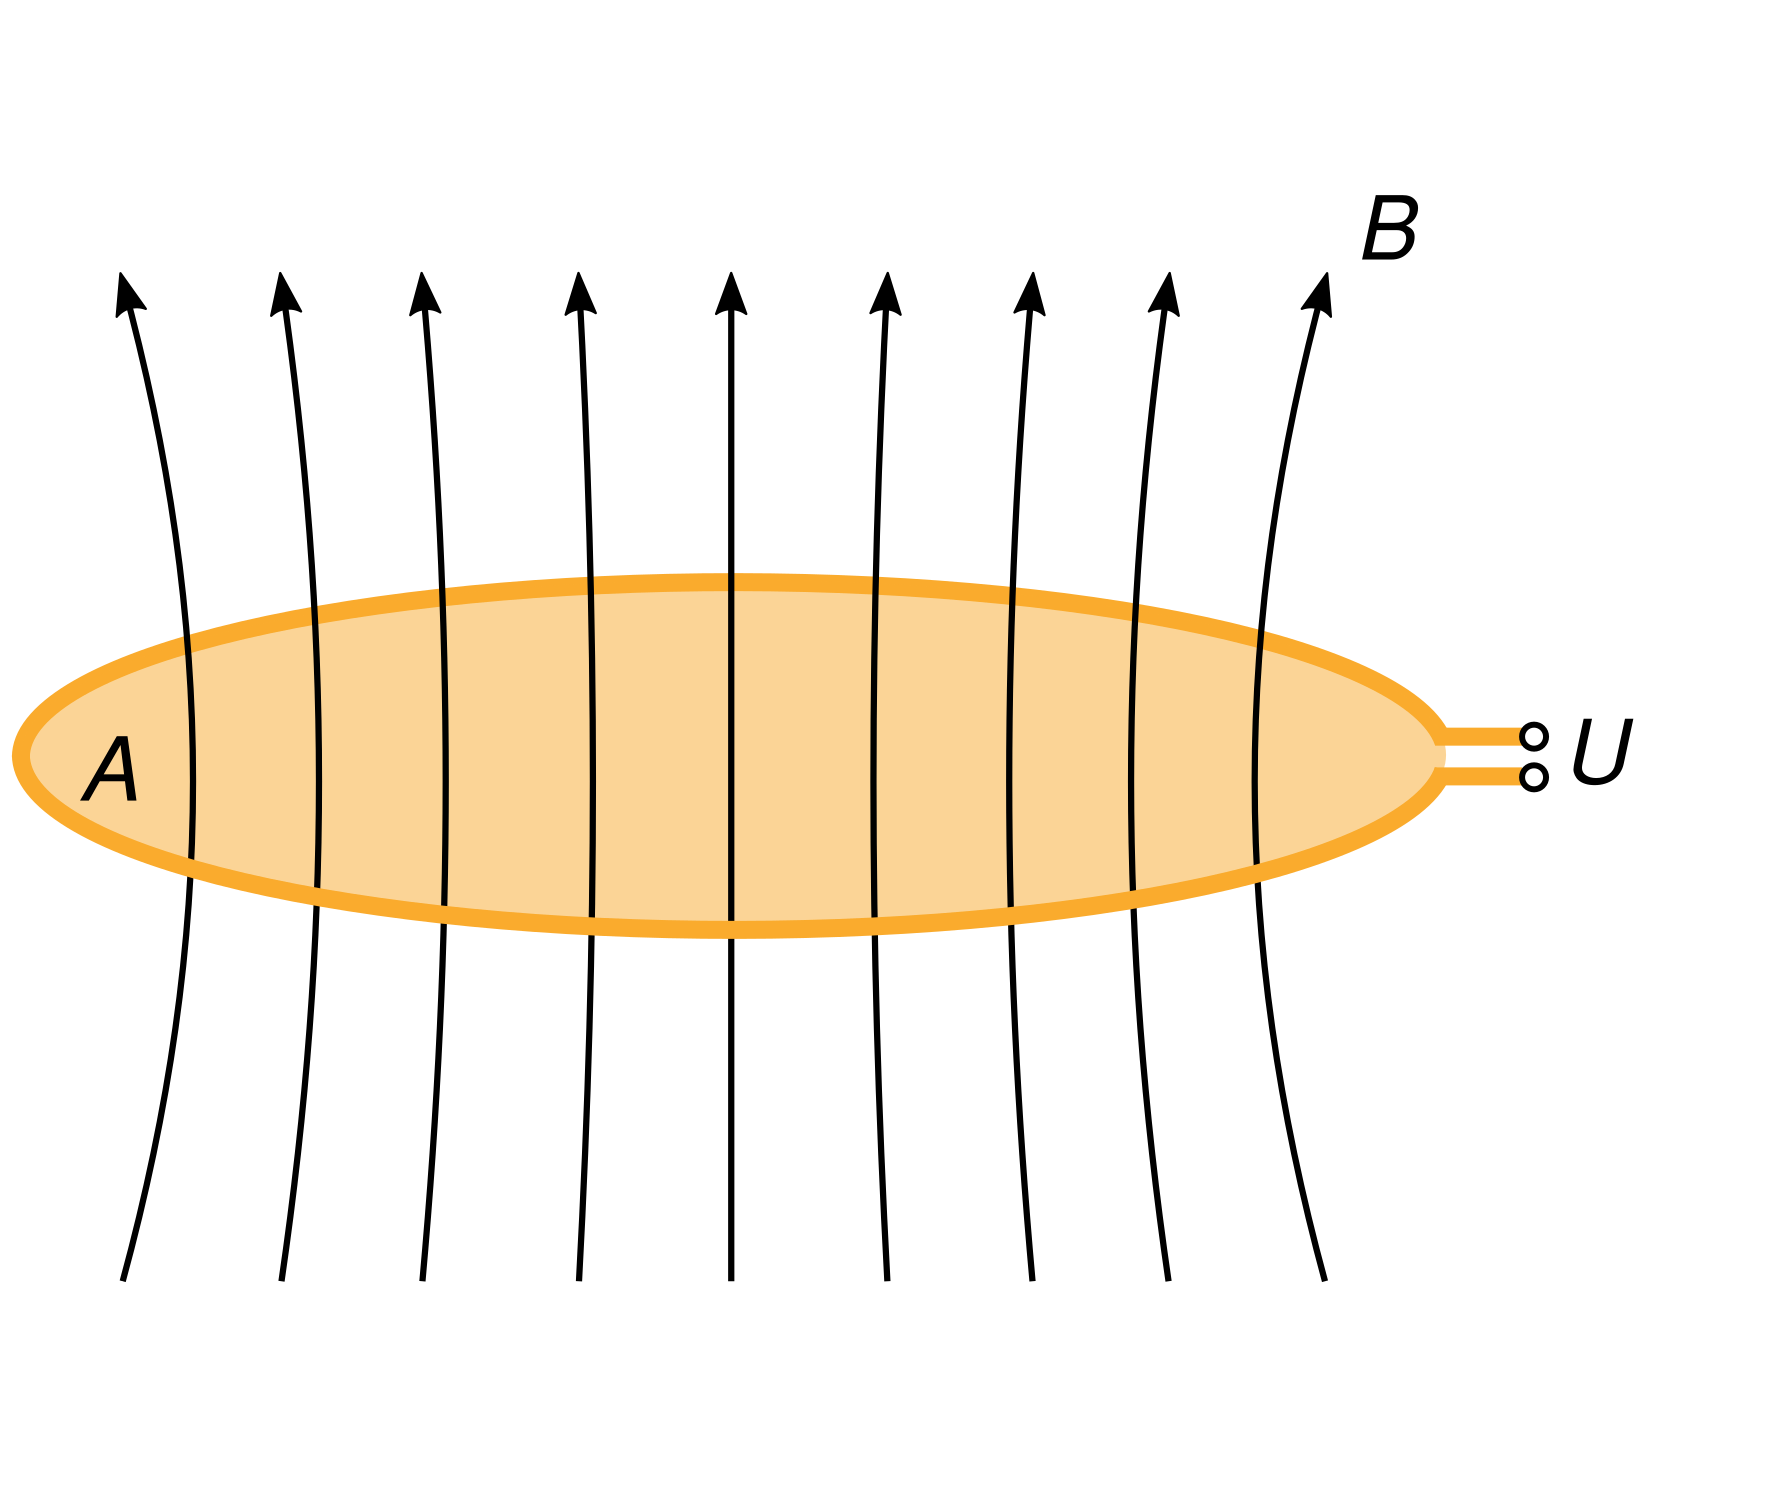
\includegraphics{appendix_methods_vsm_flux}
      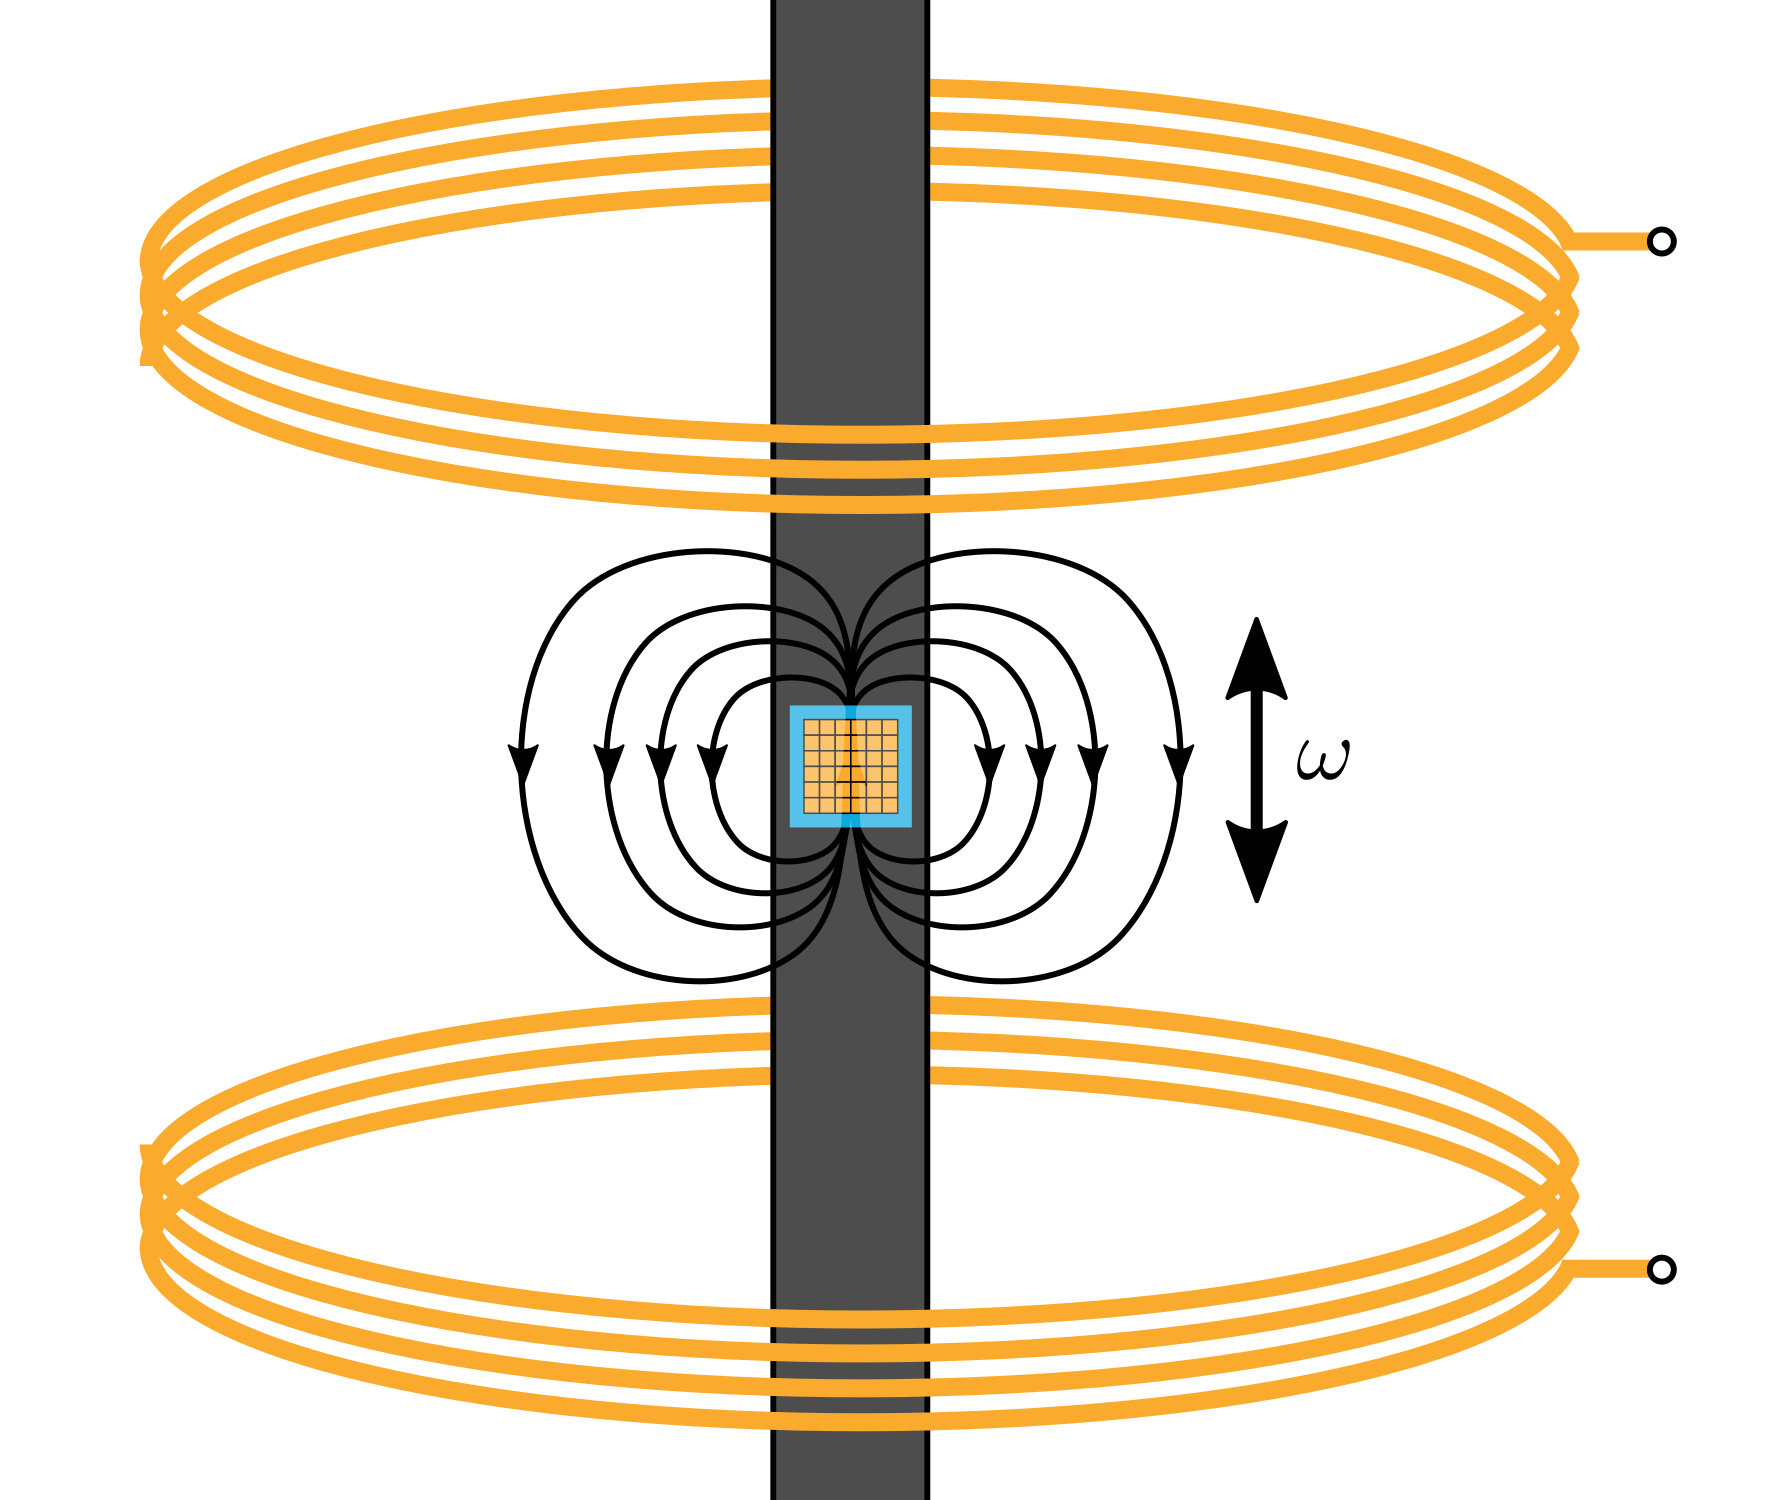
\includegraphics{appendix_methods_vsm_sample}
      \caption{\label{fig:methods:vsm:flux}Depiction of Faraday's law of induction for a single current loop (left) with cross-section $A$ being passed by a magnetic field $B$. A change in passing magnetic field creates a voltage with a magnitude equal to the change in magnetic flux. VSM uses this principle by placing a sample within a coil and vibrating it to produce a electric signal from the sample magnetization (right).}
    \end{figure}
    The magnetic flux is given by the product of the magnetic field times the area that is enclosed by the wire loop as depicted for a single current loop in \reffig{fig:methods:vsm:flux} on the left.
    Vibrating sample magnetometry uses this fundamental principle of electrodynamics to measure the magnetization by placing a small magnetic sample on a vibrating rod.
    The sample is magnetized via a constant external field $B$ and vibrates periodically with a small amplitude and defined frequency $\omega$.
    The periodic movement of the magnetized sample results in a slight periodic change of the magnetic field that passes through pickup coils placed around the sample and therefore by Faraday's induction law in a periodic voltage that can be measured and enhanced by a lock-in amplifier.
    The lock-in amplifier filters the electric signal for the specific frequency by multiplying the electric signal with a known signal having the same frequency $\omega^\prime \eq \omega$.
    By using a trigonometric identity, the mean signal measured over one period is thereby transformed to
    \begin{align}
      \begin{split}
        \braket{A \sin(\omega t) \sin(\omega^\prime t)}
          &\eq \braket{\frac{A}{2} \biggl[ \cos\Bigl((\omega - \omega^\prime) t \Bigr) - \cos\Bigl((\omega + \omega^\prime) t\Bigr) \biggr]}\\
          &\,\stackrel{\omega \eq \omega^\prime}{=}\, \frac{A}{2} \braket{1 - \cos(2\omega t)} \eq \frac{A}{2}\\
      \end{split}
    \end{align}
    such that the amplitude of the electric signal at the vibration frequency is automatically obtained by measuring the mean electric signal after the lock-in amplifier.
    By calibrating the instrument with a reference sample (typically a well characterized nickel sample), the electric signal is finally translated to a magnetic moment.
    In this thesis, the macroscopic magnetization of the samples is measured with respect to an external magnetic field and with respect to the temperature using a PPMS Evercool II instrument described in \refsec{ch:instruments:laboratoryInstruments:vsm}.

    The measured magnetization is the sum over all average magnetic moments components along the measurement coilset normal $\mu_{z,\,i}$  within the sample
    \begin{align}
      \tilde{M} \eq \sum_i \braket{\mu_{z,\,i}},
    \end{align}
    and is therefore in units $\unit{emu}$ (cgs) or $\unit{Am^2}$ (SI), where the conversion factor from one unit system to the other is $1 \unit{emu} \eq 10^{-3} \unit{Am^2}$.
    To have the magnetization in comparable units across samples, it is normalized to the volume of the magnetic material $V_\mathrm{mag}$
    \begin{align}
      M \eq \frac{\tilde{M}}{V_\mathrm{mag}}.
    \end{align}
    The conversion from the unit $\unit{memu}$ typically measured on VSM instruments, to the volume magnetization unit $\unit{\frac{kA}{m}}$ is simple when the magnetic volume is given in $\unit{mm^3}$ or equivalently $\unit{\musf L}$
    \begin{align}
      1 \unit{\frac{memu}{\musf L}} \eq 1 \unit{\frac{kA}{m}}.
    \end{align}

    A difficulty arises, however, in determining the magnetic volume $V_\mathrm{mag}$ when measuring thin layers of magnetic nanoparticles or a nanoparticle dispersion.
    It is possible to estimate the volume by trying to measuring the weight and estimating the density of the materials from bulk properties, but this is connected with large uncertainties.
    As the single particle volume $V_\mathrm{p}$ can be accurately determined by a complementary experiment such as SAXS, one can express the magnetic volume by $V_\mathrm{mag} \eq N V_\mathrm{p}$, where $N$ is the number of particles.
    Assuming the nanoparticle is in the superparamagnetic phase and non-interacting, the measured magnetization on VSM is given by a Langevin curve as described in \refapp{ch:appendix:calculations:magnetizationClassicalSpin}.
    The volume magnetization for a sample of $N$ magnetic nanoparticles is then written as
    \begin{align}
      M (H)\eq \frac{N \mu}{N V_\mathrm{p}}
      \biggl( \coth\Bigl(\frac{\mu \mu_0 H}{k_B T} \Bigr) - \frac{k_B T}{\mu \mu_0 H} \biggr).
    \end{align}
    Thus by the Langevin model, the number of particles cancels in the equation and by defining the saturation magnetization as
    \begin{align}
      \label{eq:methods:vsm:MsDefinition}
      M_s \eq \frac{\mu}{V_\mathrm{p}},
    \end{align}
    the Langevin behaviour is written as
    \begin{align}
      \label{eq:methods:vsm:scaleMagnetization}
      M(H) \eq M_s
       \biggl( \coth\Bigl(\frac{\mu \mu_0 H}{k_B T} \Bigr) - \frac{k_B T}{\mu \mu_0 H} \biggr) + \chi \mu_0 H.
    \end{align}
    In a realistic experiments, an excess susceptibility $\chi$ can arise, which manifests as a linear background and is therefore included in formula.

    This function can be fit to a given set of magnetometry data, where $M_s$, $\mu$ and $\chi$ are parameters, while $V_p$ is determined by SAXS.
    The fitted value of $M_s^\mathrm{fit}$ can be compared with \refeq{eq:methods:vsm:MsDefinition}, to obtain the scale factor that needs to be applied to the data
    \begin{align}
      \mathrm{scale} \eq \frac{1}{V_\mathrm{mag}} \eq \frac{\mu}{V_\mathrm{p} M_s^\mathrm{fit}},
    \end{align}
    which gives the magnetization scaled to the total magnetic sample volume.
\end{document}